\chapter{Case Study}

\iffalse 
$L1$ is a simple call-by-value functional language with high order functions. All functions are currified, that is, have exactly one argument.

\begin{figure}
  \caption{$L1$ Abstract Syntax}
  \begin{openframe}
    \begin{align*}
      e ::= & \quad n \quad |\quad x \quad | \quad e_1 \: op \: e_2 \\
        & |\quad \text{if } e_1 \text{ then } e_2 \text{ else } e_3 \\
        & |\quad e_1 e_2 \\
        & |\quad \text{fn x } \Rightarrow e \\
        & |\quad \text{let y } = e_1 \text{ in } e_2 \\
        & |\quad \text{letrec y } = (\text{fn x } \Rightarrow e_1) \text{ in } e_2 \\
    \end{align*}

    where

    \begin{align*}
      n & \in \mathbb{N} \\
      x & \in \text{set of variable identifiers} \\
      op & \in \{+, -, *, /,  =, <, >, \geq, \leq \} \\
    \end{align*}
  \end{openframe}
\end{figure}

Acqua goal is to explore parallel execution of function applications. A classical example that allows to explore parallel function applications is the algorithm to find the n-th number of the Fibonacci sequence. The Fibonacci number sequece starts with the number 1 two times, and all other numbers are the result of the sum of the last two numbers. Thus, the sequence is \{1,1,2,3,5,8,13,...\}.

The figure \ref{fig:fib-l1} shows a naive $L1$ program that finds the 7th number on the Fibonacci sequence. The recursive function fibo is declared on the first line. The second line shows that fibo is a function that receives one argument (as any function on $L1$) named $x$. The lines 3-5 are the body of the function, that returns 1 when $x$ is less than 2, or the sum of two fibo applications, for $x-1$ and $x-2$. The lines 6 and 8 limit the scope of this function definition. On the line 7 we have the application of the function fibo to the number 7, thus, finding the 7th number of the Fibonacci sequence.

\begin{figure}
  \caption{Fibonacci function applied to 7}
  \begin{lstlisting}[language=l1]
letrec fibo =
  fn x =>
    if x < 2
      then 1
      else (fibo (x - 1)) + (fibo (x - 2))
in
  fibo 7
end
  \end{lstlisting}
  \label{fig:fib-l1}
\end{figure}

To find the 7th Fibonacci number, we need to first find the 6th and 5th numbers. And for the 6th, we need the 5th and 4th numbers. We can represent this dependency using a tree, as show in figure \ref{fig:fibo}. This tree will have the height of $n-2$, except when we are calculating the first and second numbers of fibonacci sequence. This is so because for any node, the subtree on the right is contained on the subtree on the left. So to find the height we only need to consider the leftmost path. The width of this tree is the own fibonacci number. This is so because the width of the first and second numbers are 1, and the width of $n$ is the width of $(n-1) + (n-2)$.

\begin{figure}
    \caption{Fibonacci sequence tree}
    \centerline{
      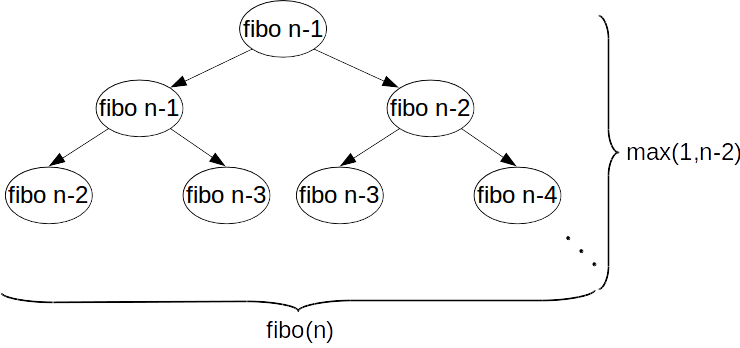
\includegraphics[width=0.7\textwidth]{fibo.png}
    }
    \label{fig:fibo}
\end{figure}

Each node in the Fibonacci dependency tree represents a function application in the program shown on figure \ref{fig:fib-l1}. The acqua architecture allows function applications to be done in parallel, so the architecture has the potential to parallelize the width of the tree in a given moment, that is $fibo(n)$ function applications. Function application will generate a job, and each job will potentially copy one environment with only two name bindings: The $x$ variable and the reference to $fibo$ function, thus the environment copy is constant. Assuming that we have enough processing units in the architecture, we can execute the naive program shown on figure \ref{fig:fib-l1} in linear time.
\fi
